\section{Machine learning\label{ml}}
\subsection{Decision trees} 
As mentioned in Section \ref{ml-bg}, AdaBoost 
with decision trees was the algorithm of choice for \nr{}'s news
personalisation.  The algorithm was applied to several tasks:
\begin{enumerate}
    \item Determining which Wikipedia webpages correspond to news sources.
    \item Finding the official homepage of a news source from a
          wikipedia webpage.
    \item Determining if a webpage is a news index.
    \item Determining if a webpage is a news item.
    \item Personalising the selection of articles a user sees.
\end{enumerate}
\paragraph{Decision thresholds} Depending on the task, different {\it decision thresholds}
were used.  Moving this threshold closer to zero increases recall at the cost of precision.  Moving
the threshold closer to one increases precision at the cost of recall.  F1 tends to peak
around the point where precision and recall are most similar.

In the task of identifying official homepages, a minimum precision score of 95\% was set.
\begin{figure}[H]
    \centering
    \fbox{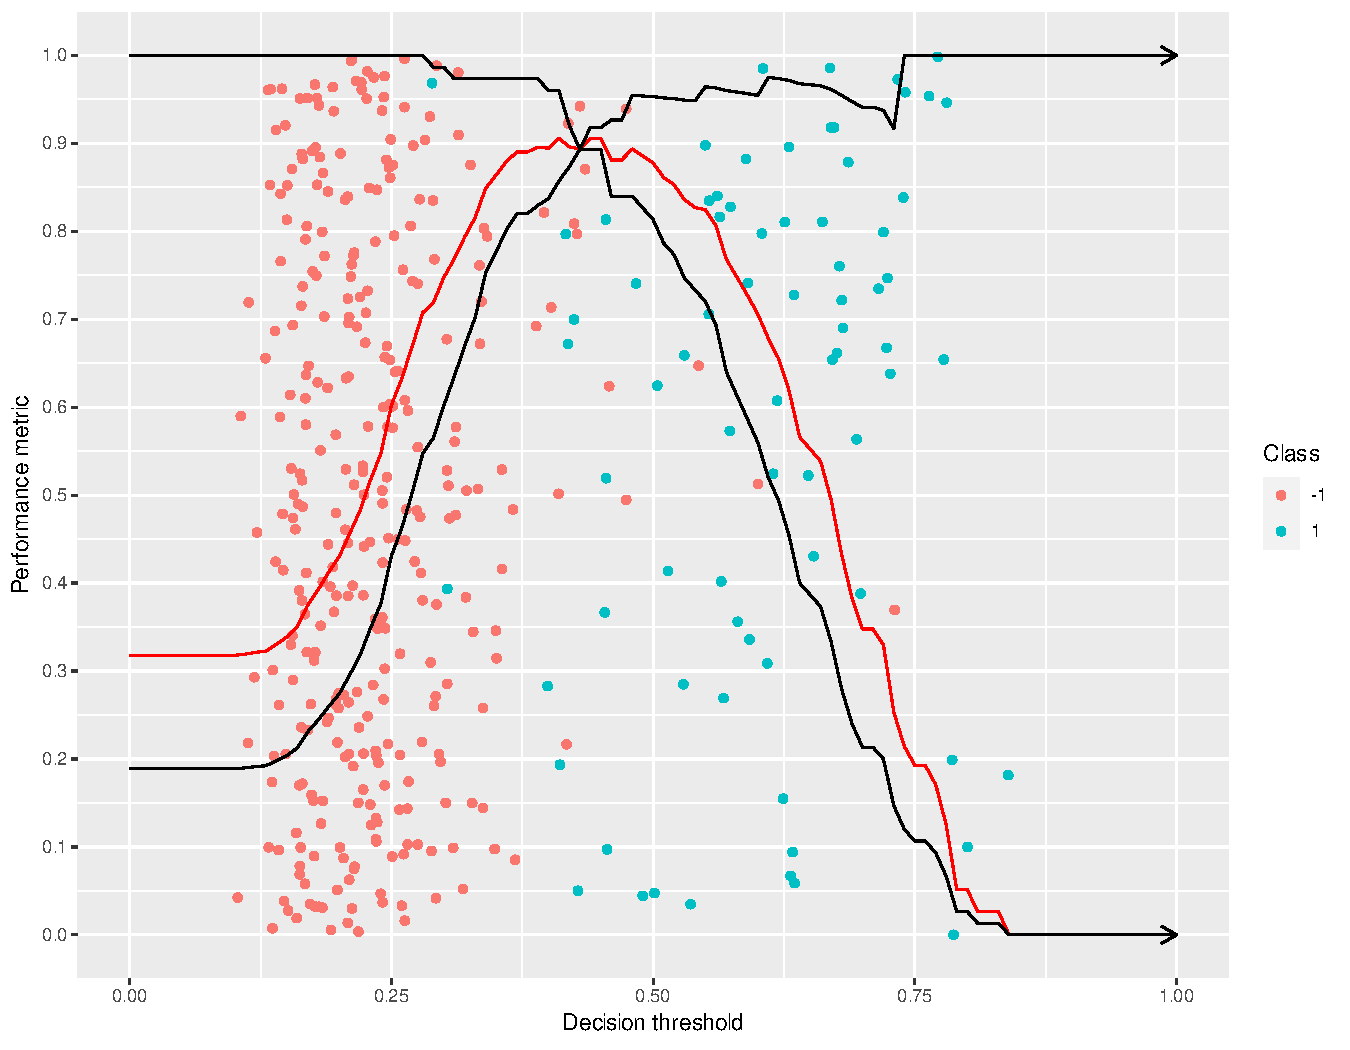
\includegraphics[width=0.8\textwidth]{media/dt.pdf}}
    \caption{
        \raggedright
        Comparing the effects of decision threshold choices (the descending black line is recall,
            the ascending black line is precision, and the curved red line is F1 score).\label{dt_cmp}
    }
\end{figure}
\subsection{Bayesian classifiers}
Although bayesian classifiers aren't as powerful as decision trees,
they are simple and efficient, and they do play their part in certain
parts of the \nr{} application.  For example, a classifier that determine
if different newspapers might be from the same geographical region
uses Bayesian classification with a few pre-labelled newspapers.  Although
this is supervised learning, the labelling is trivial, since \nr{}
currently only supports news from 6 countries.
\subsection{Feature engineering}
Traditional computer science algorithms played their part in feature
engineering, particularly in the task of identifying a news source's
homepage from its Wikipedia article.  As mentioned in Section \ref{subd},
the sub-documents file is made up of all the leaf nodes in a HTML file's
DOM.  For anchors, the left hand side of a sub-document will contain
attributes for the text and the {\tt href}.  The domain name is extracted
from the {\tt href}.  Next, two features are built, firstly by comparing
domain to the last part of the current resource's path, and secondly by comparing the
anchor's text to the last part of the path.  This comparison uses
the Levenshtein distance ($LD$) between two strings \cite{levenshtein1966},
and normalises
the distance to a scale between 0 and 1 (0 being low similarity, and
1 being high similarity).  This normalisation is carried out as follows:
\begin{equation}
    Similarity(a, b) = 1 - \frac{LD(a, b)}{max(|a|, |b|)}
\end{equation}
Normalisation fills two purposes here.  Firstly, it makes
separate results from $LD$ somewhat comparable.  E.g.
two 100,000 word texts with 6 differences will no longer have the same
difference/similarity score as the score between `\underline{newspa}per' and
`\underline{zookee}per'.  In other words, the size of the texts being compared will
normalise the similarity score.  Secondly, plotting similarity from
0 to 1 is convenient for decision tree algorithms, and it's also convenient
(in the case of \nr{}) to place the {\it similarity} end closer to 1 than to 0.
This is because \nr{}'s DT implementation uses a default of 0 when a feature
is missing from a document or sub-document.

\subsection{Training\label{training}}
The training data for the decision trees are
assembled from the {\tt likes} and {\tt dislikes} of the user.
The \nr{} website stores the data on the user's side, and the
data is assembled through the display of an upvote
and downvote button alongside each news item.
Section \ref{privacy} outlines how this is accomplished using
web browser technology.
\subsection{Predicting\label{predicting}}